\subsection{Licht und Wahrnehmung}
Beantworten Sie folgende Fragen zum Thema Licht und Wahrnehmung.
\begin{enumerate}
    \item   \question{In welchem Wellenlängenbereich der elektromagnetischen Strahlung kann das menschliche Auge Licht wahrnehmen?}\\\\
            Der Bereich liegt zwischen $\SI{380}{nm}-\SI{780}{nm}$.

    \item   \question{Bei welcher Wellenlänge liegt die größte Hellempfindlichkeit für\\ a) Tagsehen \\b) Nachtsehen}\\\\
            $\SI{550}{nm}$ und $\SI{505}{nm}$ respektive.

    \item   \question{Was versteht man unter Akkomodation des Auges?}\\\\
            Die Akkomodation ermöglicht eine Veränderung der Brennweite. Somit kann das Auge auf ein
            näheres Objekt fokussieren.

    \item   \question{Was versteht man unter Adaption des Auges und welche Abläufe im Auge ermöglichen die Adaption?}\\\\
            Anpassung an Lichtvehältnissen. Die Iris wirkt wie eine Blende bei handelsüblichen Kameraapparaten. Sie kann sich für helle Szenen 
            zusammenziehen und bei dunklen Szenen weiten.

    \item   \question{Wie entstehen die Farben aus den Grundfarben über additive Farbmischung?}\\\\
            Ausgehend von Schwarz werden (Grund-)Farben hinzugefügt bis die gewünschte Farbe erreicht wird.
    \item   \question{Wie entstehen die Farben aus den Grundfarben über subtraktive Farbmischung?}\\\\
            Ausgehend von einem definierten Frequenzspektrum (alle Freq.: Weiß) werden Farben (Frequenzen) abgezogen 

    \item   \question{Was versteht man in der Lichttechnik unter einem kontinuierlichen Spektrum. Nennen Sie Beispiele für Lichtquellen mit kontinuierlichem Spektrum.} \\\\
            Tageslicht hat eine durchgängige spektrale Strahlungsverteilung: Ein kontinuierliches Spektrum. Nur Temperaturstrahler (Glühlampen, Halogenlampen) weisen ein kontuierliches Spektrum auf.
            \begin{figure}[!hpt]
                \centering
                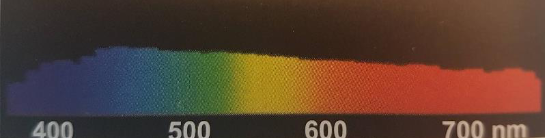
\includegraphics{img/Spektrum_des_Tageslichts.png}
                \caption{Spektrum des Tageslichtes}
            \end{figure}

    \item   \question{Was versteht man in der Lichttechnik unter einem diskreten Spektrum? Nennen Sie Beispiele für Lichtquellen mit diskretem Spektrum.}\\\\
            Ein diskretes Spektrum weist eine unterschiedliche spektrale Verteilung auf. Beispiele sind Entladungslampen.
            \begin{figure}[!hpt]
                \centering
                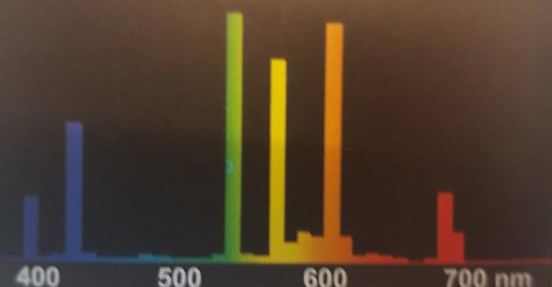
\includegraphics{img/Spektrum_einer_Quecksilberdampg-Hochdrucklampe.png}
                \caption{Spektrum einer Quecksilberdampf-Hochdrucklampe}
            \end{figure} 

    \item   \question{Was versteht man unter Farbtemperatur: Wie ist sie definiert und in welcher Einheit wird sie angegeben?}\\\\
            Sie ist ein Maß, um den Farbeindruck einer Lichtquelle zu beschreiben. Die Einheit der Farbtemperatur ist Kelvin. Darunter versteht man ebenfalls jene Glühtemperatur, auf die man den „schwarzen Körper“ bringen müsste, damit er Licht gleicher Farbe aussendet wie die zu untersuchende Lichtquelle.


    \item   \question{Was versteht man unter dem Farbwiedergabeindex (CRI) $R_a$? Wie wird der Farbwiedergabeindex berechnet?}\\\\
            Der Farbwiedergabeindex gibt an, wie farbecht Farben unter künstlichem Licht dargestellt werden.
            Der CRI wird berechnet, indem die Farben von acht Standardfarben unter der zu testenden Lichtquelle mit den Farben unter einer Referenzlichtquelle verglichen werden.

    \item   \question{Was bedeutet eine Kennzeichnung mit den drei Ziffern 950 auf dem Sockel eines Leuchtmittels?}\\\\
            Das Leuchtmittel weist eine Farbwiedergabestufe von A1 (90\%) sowie eine Farbtemperatur von $\SI{5}{kK}$ auf. Es wird als 
            Neutralweiß bezeichnet.
\end{enumerate}

\subsubsection{Lichttechnische Größen}
Arbeiten Sie folgende Aufgabenstellung genau und zielführend durch:

\begin{enumerate}
    \item   \question{Nennen sie die vier lichttechnischen Grundgrößen und ihre Einheiten sowie die Bedeutung dieser Größen.} \\\\
            
            Es wird zwischen folgenden Größen unterschieden:
            \begin{itemize}
                \item \textbf{Lichtstrom $\phi$}: $\left[\phi\right] = \textnormal{lm}$ \\ Die gesamte von einer Lichtquelle abgegebene und vom Auge bewertete Strahlungsleistung. Durch Lampenhersteller angegeben.
                \item \textbf{Lichtstärke $I$}: $\left[I\right] = \textnormal{cd}$ \\ Sie ist ein Maß für die Intensität des Lichts in einer bestimmten Richtung.
                \item \textbf{Beleuchtungsstärke $E$}: $\left[E\right] = \textnormal{lx}$ \\ Sie ist das Verhältnis von Lichtstrom zur Fläche, auf die der Lichtstrom auftritt
                \item \textbf{Leuchtdichte $L$}: $\left[L\right] = \frac{cd}{m^2}$
            \end{itemize}

    \item   \question{Wie heißt die lichttechnische Größe und Einheit, mit der die gesamte, von einer Lichtquelle abgegebene und vom Auge bewertete Strahlungsleistung gemessen wird?} \\\\
            Die Größe ist der Lichtstrom $\phi$. Es gilt: $\left[\phi\right] = \textnormal{lm}$

    \item   \question{Wie errechnet sich die Lichtausbeute einer Lichtquelle (Formel angeben)?}
            $$\textnormal{Lichtausbeute} = \frac{\phi}{P}$$

    \item   \question{Auf welche lichttechnische Größe bezieht sich die Energieeffizienzklasse, die entsprechend der EU-Richtlinie auf der Verpackung von Leuchtmitteln angegeben ist?} \\\\
            Die Energieeffizienzklasse bezieht sich auf die Lichtausbeute.

    \item   \question{Wie heißt die lichttechnische Größe und Einheit, mit der die gesamte, auf einer Fläche auftreffende und vom Auge bewertete Strahlungsleistung $\phi$ im Verhältnis zur Flächengröße gemessen $A$ wird?}\\\\
            Beleuchtungsstärke $E$
    \item   \question{Wie errechnet sich die Beleuchtungsstärke aus $\phi$ (Formel angeben)?}
            $$E = \frac{\phi}{A}$$
    \item   \question{Wie errechnet sich die horizontale Beleuchtungsstärke aus $I$?}
            $$E_H= \frac{\vec{I}}{h^2} \cdot \cos^3\left(\alpha\right)$$ \Huge MAYBE TODO. IDK. \normalsize
    \item   \question{Wie errechnet sich die vertikale Beleuchtungsstärke aus $I$?}
            $$E_V = \frac{\vec{I}}{r^2} \cdot \sin \left(\alpha\right)$$
    \item   \question{Was ist eine Lichtverteilungskurve? Erklären Sie anhand der C-Ebene den Zusammenhang zwischen Lichtverteilungskurve und Lichtverteilungskörper.}\\\\
            Mit den Lichtstärkeverteilungskurven einer Lampe oder Leuchte kann man die Lichtstärke für
            beliebige Raumwinkel darstellen.
            
    \item   \question{Erklären Sie den Zusammenhang zwischen Lichtstrom und Lichtstärke.}
            $$I_V = \frac{\textnormal{d}\Phi_V}{\textnormal{d}\Omega}$$

            $\Phi$ ... gesamter Lichtstrom der Lichtquelle\\
            $\textnormal{d}\Omega$ ... differentieller Raumwinkel\\
            $\Phi_V$ ... Lichtstrom der Lichtquelle in Richtung des differentiellen Raumwinkels

    \item   \question{Wie groß ist die Beleuchtungsstärke, wenn ein Lichtstrom $\Phi = \SI{800}{lm}$ gleichmäßig und normal auf eine Fläche von $A = \SI{6}{m^2}$ auftrifft?}
            $$E = \frac{\Phi}{A} = \frac{\SI{800}{lm}}{\SI{6}{m^2}} = \SI{133.3}{lx}$$
\end{enumerate}

